Since the one-dimensional spherical base state is not aligned with the
3-d Cartesian grid we use for full star spherical geometry, computing quantities that
involve both the base state and the full state becomes complicated.
Therefore, various parts of the algorithm (such as the averaging operations)
require a mapping between the base state and the full state.

As there is no alignment between the 3-d Cartesian grid and the 1-d
spherical base state grid, we are free to choose their grid spacings
independently.  Experimentation has shown that the best choice results
from picking the 3-d Cartesian grid spacing, $\Delta x,$ to be coarser
than the 1-d spherical base state spacing, $\Delta r$.  (Here we
assume $\Delta x = \Delta y = \Delta z.$)  For the paper IV simulations,
we use $5 \Delta r = \Delta x$.  We refer to the procedure that maps data 
from 1-d to 3-d as {\tt fill\_3d}, and the
complementary procedure that maps from 3-d to 1-d as {\tt average}.
\section{\tt fill\_3d}
There are two different {\tt fill\_3d} modes, each performed with the
subroutine, {\tt put\_1d\_array\_on\_cart}:
\begin{enumerate}
\item The 1D array is cell-centered, and we map to Cartesian cell-centers.  
This is the most commonly used mode of {\tt fill\_3d}, and in paper IV, 
we refer to this mode as {\tt fill\_3d}.
\item The 1D array is edge-centered, and we map to Cartesian cell-centers.
\end{enumerate}
\subsection{1D Cell-Centered to Cartesian Cell-Centered}
\label{Sec:1D Cell-Centered to Cartesian Cell-Centered}

Figure  \ref{fig:mapping} shows the Cartesian grid overlaid by the 
spherical base state (for simplicity, the figure is drawn in 2-d 
using $2 \Delta r = \Delta x$).
The {\tt fill\_3d} procedure computes the distance of the center of
cell indexed by $(i,j,k)$ from the center of the star,
\begin{equation}
r = \sqrt{(x_i - x_c)^2 + (y_j - y_c)^2 + (z_k - z_c)^2},
\end{equation}
where $(x_c, y_c, z_c)$ are the coordinates of the center of the star.
We use this radius to find the corresponding radial bin as $n = \mathtt{int}(r
/ \Delta r)$ (here, our convention is to use 0-based indexing for the
base state).  We can then initialize a Cartesian cell quantity $q$ from its
corresponding base state quantity, $q_0,$ as $q_{i,j,k} = q_{0,n}$.

In essence, we are doing a piecewise constant interpolation of the radial array 
onto the Cartesian grid.  If the output is a vector quantity, rather than a 
scalar, we multiply the result by the unit vector in the normal direction.
\subsection{1D Edge-Centered to Cartesian Cell-Centered}
\label{Sec:1D Edge-Centered to Cartesian Cell-Centered}
Again, for each Cartesian cell-center, we compute the corresponding radial
bin.  We linearly interpolate from the two nearest radial edge values 
to get the Cartesian cell-centered value.  In essence,
we are doing a piecewise linear interpolation of the radial array onto the 
Cartesian grid.  If the output is a vector quantity, rather than a scalar, we
multiply the result by the unit vector in the normal direction.
We use this function for:
\begin{enumerate}
\item Putting $\nabla p_0$ from radial edges onto cell centers as a vector.
\item Computing radial velocity for plotfile.
\end{enumerate}
\section{1D Edge-Centered to Cartesian Edges}
\label{Sec:1D Edge-Centered to Cartesian Edges}
This case is only used to create {\tt w0mac} from {\tt w0} in the 
subroutine, {\tt put\_w0\_on\_edges}.  There are several variations 
of the interpolation, controlled by {\tt w0mac\_interp\_type}.  We 
currently use the default, {\tt w0mac\_interp\_type} = 1.  We first 
map $w_0$ onto Cartesian cell-centers, and multiply the result by 
the unit vector in the normal direction.  Then, for each Cartesian 
face, we obtain the normal velocity by averaging the corresponding 
velocities from the Cartesian cell-centers adjacent to the face.
\section{1D Cell-Centered to Cartesian Edges}
At various points in the algorithm we need to map cell-centered radial 
quantities onto Cartesian edges.  For example, we need $\rho_0$ at edges 
to compute the full state $\rho$ used to compute fluxes.  What we do
is call {\tt fill\_3d}, and then average neighboring cell-centers onto
edges.
\section{{\tt average}}\label{Sec:Avg}
For the {\tt average} process, we first define a coarse 1-d radial array 
with $\Delta r_{\rm c} = \Delta x$.  Then, for each cell indexed by
$(i,j,k)$ we again compute the radius, $r,$ as above, and 
define the index of the corresponding coarse radial bin, 
$n_{\rm c} = \mathtt{int}(r / \Delta r_{\rm c})$.  
We define $q_{0,n_{\rm c}}$ as the average of all the $q_{i,j,k}$ whose 
Cartesian cell centers map into coarse radial bin $n_{\rm c}$.
Next, we construct edge-centered states on the coarse radial bin using 
the fourth order approximation,
$q_{0,n_{\rm c}+\myhalf} = (7/12)(q_{0,n_{\rm c}}+q_{0,n_{\rm c}+1}) 
- (1/12)(q_{0,n_{\rm c}-1}+q_{0,n_{\rm c}+2})$.  Finally, for each coarse radial bin
we construct a quadratic profile using $q_{0,n_{\rm c}-\myhalf}, q_{0,n_{\rm c}}$ 
and $q_{0,n_{\rm c}+\myhalf}$.  This is based on the interpolating polynomial used by 
the PPM scheme to find edge states (Colella \& Woodward 1984).  Specifically, for 
$n_{\rm c}\Delta r_{\rm c} \le r \le (n_{\rm c}+1)\Delta r_{\rm c}$, the 
interpolating polynomial is
\MarginPar{Need to add description of limiters}
\begin{equation}
q_0(r) = q_{0,n_{\rm c}-\myhalf} + \xi(r)\left\{\Delta q_{n_{\rm c}} + q_{6,n_{\rm c}}[1 - \xi(r)]\right\},
\end{equation}
with
\begin{equation}
\xi(r) = \frac{r - n_{\rm c}\Delta r_{\rm c}}{\Delta r_{\rm c}},
\end{equation}
\begin{equation}
\Delta q_{n_{\rm c}} = q_{0,n_{\rm c}+\myhalf} - q_{0,n_{\rm c}-\myhalf},
\end{equation}
and
\begin{equation}
q_{6,n_{\rm c}} = 6\left[q_{0,n_{\rm c}} - 
\frac{1}{2}\left(q_{0,n_{\rm c}+\myhalf} + q_{0,n_{\rm c}-\myhalf}\right)\right].
\end{equation}

\subsection{Mapping}
\begin{equation}
\left.\begin{array}{cccccccc}
\bf{r} & \text{r\_cc\_loc} & \text{number at distance} & \text{i offset} & \text{j offset} & \text{k offset} & \text{exact dist} & \text{approx dist} \\
\hline
0 & 0.1 & 0 & & & & & \\
1 & 0.3 & 0 & & & & & \\
2 & 0.5 & 0 & & & & & \\
3 & 0.7 & 0 & & & & & \\
4 & 0.9 & 8 & 0.5 & 0.5 & 0.5 & \sqrt{3/4} & 0.866 \\
5 & 1.1 & 0 & & &  & &\\
6 & 1.3 & 0 & & & & & \\
7 & 1.5 & 0 & & & & & \\
8 & 1.7 & 24 & 0.5 & 0.5 & 1.5 & \sqrt{11/4} & 1.658\\
9 & 1.9 & 0 & & & & & \\
10 & 2.1 & 24 & 0.5 & 1.5 & 1.5 & \sqrt{19/4} & 2.179 \\
11 & 2.3 & 0 & & & & & \\
12 & 2.5 & 32 & 0.5 & 0.5 & 2.5 & \sqrt{27/4} & 2.598 \\
13 & 2.7 & 0 & & & & & \\
14 & 2.9 & 48 & 0.5 & 1.5 & 2.5 & \sqrt{35/4} & 2.958 \\
15 & 3.1 & 0 & & & \\
16 & 3.3 & 24 & 1.5 & 1.5 & 2.5 & \sqrt{43/4} & 3.279 \\
17 & 3.5 & 48 & 0.5 & 0.5 & 3.5 & \sqrt{51/4} & 3.571 \\
18 & 3.7 & 0 & & & & & \\
19 & 3.9 & 72 & 0.5 & 1.5 & 3.5 & \sqrt{59/4} & 3.841 \\
20 & 4.1 & 24 & 1.5 & 1.5 & 3.5 & \sqrt{67/4} & 4.093 \\
21 & 4.3 & 56 & 0.5 & 2.5 & 3.5 & \sqrt{75/4} & 4.330 \\
22 & 4.5 & 72 & 0.5 & 0.5 & 4.5 & \sqrt{83/4} & 4.555 \\
23 & 4.7 & 48 & 0.5 & 1.5 & 4.5 & \sqrt{91/4} & 4.770 \\
24 & 4.9 & 72 & 1.5 & 1.5 & 4.5 & \sqrt{99/4} & 4.974 \\
25 & 5.1 & 72 & 0.5 & 2.5 & 4.5 & \sqrt{107/4} & 5.172 \\
26 & 5.3 & 48 & 1.5 & 2.5 & 4.5 & \sqrt{115/4} & 5.362 \\
27 & 5.5 & 48 & 0.5 & 0.5 & 5.5 & \sqrt{123/4} & 5.545 \\
28 & 5.7 & 120 & 0.5 & 1.5 & 5.5 & \sqrt{131/4} & 5.723 \\
29 & 5.9 & 72 & 1.5 & 1.5 & 5.5 & \sqrt{139/4} & 5.895 \\
30 & 6.1 & 56 & 0.5 & 2.5 & 5.5 & \sqrt{147/4} & 6.062 \\
31 & 6.3 & 121 & & & & \sqrt{155/4} & 6.225 \\
& & & & & & \sqrt{163/4} & 6.384 \\
\end{array}\right.
\end{equation}

\clearpage

\begin{figure}[tpb]
\begin{center}
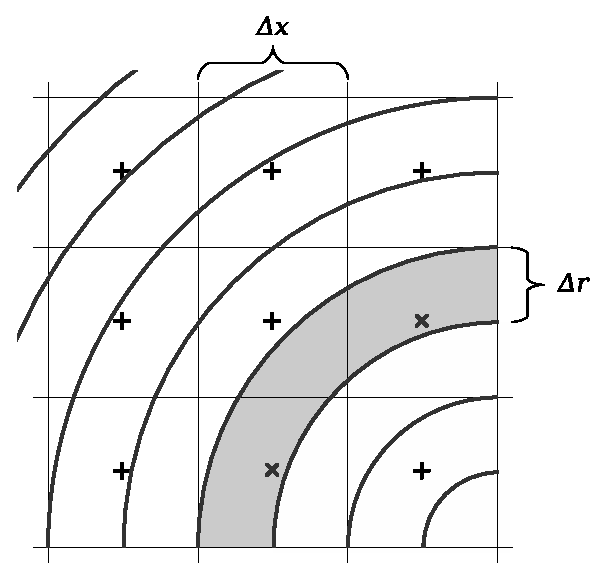
\includegraphics{\radbasefigpath/mapping2_bw}
\caption{\label{fig:mapping} The Cartesian grid and spherical base
state (shown here in 2-d for simplicity using $2 \Delta r = \Delta x$).
Here we represent the
spherical base state as concentric shells (blue lines).  Since the
base state is not aligned with the Cartesian grid we use on which
we discretize the star, we need to map between the two configurations.
The `$+$' symbols represent the Cartesian zone centers.  In our
mapping, the zone marked with the red symbol maps into the gray-shaded
radial bin. }
\label{fig:mapping}
\end{center}
\end{figure}
